\documentclass[12pt, a4paper]{article}

% ── PAQUETES ─────────────────────────────────────────────────
% Los paquetes amplían las capacidades de LaTeX.
% Se cargan en el "preámbulo" (antes de \begin{document}).

\usepackage[utf8]{inputenc}       % Permite tildes y ñ
\usepackage[spanish]{babel}       % Idioma español (guiones, fechas, etc.)
\usepackage{geometry}             % Control de márgenes
\usepackage{graphicx}             % Para insertar imágenes
\usepackage{setspace}             % Control de interlineado
\usepackage{hyperref}             % Links clicables (índice, URLs)
\usepackage{xcolor}               % Colores personalizados
\usepackage{listings}
\usepackage{tcolorbox}
\usepackage{amsmath}
\usepackage{float}
\usepackage{booktabs}
\usepackage{subcaption}
\usepackage{chngcntr}
\usepackage{array}
\usepackage{tabularx}
\usepackage{ragged2e}

\counterwithin{figure}{subsection}
\tcbuselibrary{listings, skins}

\newtcblisting{terminal}{
    colback   = black,           % fondo negro
    colframe  = gray!50,         % borde gris
    coltitle  = black,           % título en blanco
    coltext   = green!70!white,  % texto verde (estilo terminal clásica)
    title     = Terminal,
    fonttitle = \bfseries\small,
    listing only,
    listing options = {
        basicstyle = \ttfamily\small\color{green!70!white},
        breaklines = true,
    }
}

\lstset{
    basicstyle    = \ttfamily\small,   % fuente monoespaciada
    keywordstyle  = \color{blue},      % palabras clave en azul
    commentstyle  = \color{gray},      % comentarios en gris
    stringstyle   = \color{orange},    % strings en naranja
    numbers       = left,              % números de línea a la izquierda
    frame         = single,            % recuadro alrededor del bloque
    breaklines    = true,              % corta líneas largas automáticamente
}

\newcommand{\tema}{Plataforma de Verificación}
\newcommand{\titulotrabajo}{Informe}
\newcommand{\autor}{Alfici, Facundo Ezequiel}
\newcommand{\documento}{44012327}
\newcommand{\curso}{PROCOM}
\newcommand{\fundacion}{Fundación Fulgor}
\newcommand{\fecha}{\today}

% ── INICIO DEL DOCUMENTO ─────────────────────────────────────
% Todo lo visible va DENTRO de este entorno
\begin{document}

% Quitamos la numeración en la carátula
\thispagestyle{empty}

% ── CARÁTULA ─────────────────────────────────────────────────
\begin{center}   % Entorno para centrar contenido

    % --- Encabezado institucional ---
    {\Large \textbf{\fundacion}}\\[0.3cm]      % \\ fuerza un salto de línea                 % [0.2cm] = espacio extra después
    {\large \curso}

    \vspace{1.5cm}   % Espacio vertical de 1.5 cm

    % --- Logo (opcional) ---
    % Descomenta las 2 líneas siguientes si tenés un logo guardado
    % \includegraphics[width=0.25\textwidth]{logo.png}
    % \vspace{1cm}

    \hrule height 1pt   % Línea horizontal
    \vspace{0.4cm}

    % --- Título del trabajo ---
    {\LARGE \textbf{\titulotrabajo}}\\[0.3cm]
    {\large \tema}

    \vspace{0.4cm}
    \hrule height 1pt

    \vspace{2.5cm}

    % --- Datos del alumno ---
    % Tabla simple de 2 columnas: etiqueta y valor
    \begin{tabular}{r l}   % r = columna alineada a la derecha, l = izquierda
        \textbf{Autor:}   & \autor\\[0.2cm]
        \textbf{Documento:}  & \documento\\[0.2cm]
        \textbf{Docentes:} &  Ariel Pola, Santiago Garaventta Pascual y Agustín Pesce\\
    \end{tabular}

    \vspace{3cm}

    % --- Fecha ---
    {\large \fecha}

\end{center}

% Salto de página → el informe real comienza en la siguiente hoja
\newpage

% ── EJEMPLO DE PRIMERA SECCIÓN (para no dejar el doc vacío) ──
\tableofcontents   % Genera el índice automáticamente
\newpage


\section{Introducción}
En este trabajo se realizó un programa en lenguaje C, con el que se programa el MicroBlaze
que se utilizó en el trabajo, y un programa en Python que se encarga de comunicarse con la placa por
medio de la librería PySerial.
Los desafíos principales se muestran a continuación.
\begin{itemize}
    \item Controlar el led a encender o apagar (0, 1, 2 o 3). El color de cada led puede ser rojo, azul, verde o cualquier combinación de ellos
    \item Leer el estado de los switches de la placa, manejados por medio de las Virtual Input/Output
    \item Definir una trama para el envío de los datos, considerando Device y Data como se deseen.
    \item Ejemplo de desarrollo en la siguiente figura.
\end{itemize}

\begin{figure}[H]
    \centering
    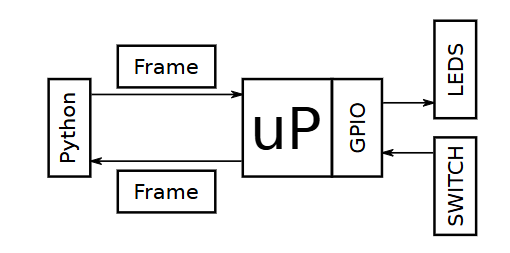
\includegraphics[width=0.7\textwidth]{imagenes/comms_example.png}
    \caption{Diagrama en bloques del flujo completo.}
    \label{fig:comms_example}
\end{figure}

\newpage

\section{Desarrollo}

\subsection{Firmware del MicroBlaze}
    En este inciso se detallará la estructura del código que conforma el firmware cargado a la FPGA, encargado de manejar el
    \textbf{MicroBlaze}. Escrito en lenguaje C, es el encargado de controlar las acciones que permiten la lectura y escritura de las entradas y
    salidas de propósito general de la FPGA.

    Utilizando las librerías \texttt{xgpio.h y xuartlite.h} se puede controlar los elementos necesarios para realizar el trabajo solicitado.
    En primera medida, se definieron los devices a leer/escribir, siendo los 4 leds y los switches de la placa.
    A los leds se les cargarán ciertos valores según el color a mostrar, permitiendo controlar el RGB de cada led a voluntad.
    Algo importante a tener en cuenta fue la selección de la trama, la cual fue dejada a consciencia del desarollador, por ello, se eligió la trama mostrada
    por el profesor, la cual se muestra en la siguiente figura.

    \begin{figure}[H]
        \centering
        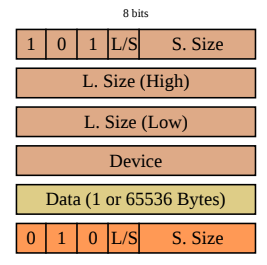
\includegraphics[width=0.5\textwidth]{imagenes/trama_type.png}
        \caption{Construcción de la trama de envío y recepción.}
        \label{fig:trama_type}
    \end{figure}

    Con esto, el programa se encargará de enviar y recibir tramas definidas por un \textbf{Header}, compuesto de una combinación de bits para indicar el inicio,
    tipo de trama, cantidad de bits de la información y el dispositivo a utilizar. Luego se envia la \textbf{Data} y se cierra el ciclo con otra combinación de bits llamada
    \textbf{Trailer o Fin de trama} que contendrá una combinación de cierre, el tipo de trama y la cantidad de bits en caso de ser corta.

    Con esto, se colocaron diferentes verificaciones dentro del código, de tal manera que si hay un corrimiento de trama debido a algun error del hardware
    o de python la trama se descarte, lo que permite mayor robustez en el comportamiento del micro.

\subsection{Programa en Python}
    En lo que respecta a la estructura del programa realizado en Python, se utilizó la librería \texttt{PySerial} para poder comunicarse con la placa por medio del puerto serial.
    La configuración se realizó a una velocidad de 115200 baudios, sin bit de paridad, 8 bits de datos y 1 bit de stop. Se definieron las funciones necesarias para poder enviar y recibir tramas,
    las cuales se encargan de construir la trama según lo definido en el firmware del microblaze.
    Estos comandos se detallan a continuación:
    \begin{itemize}
        \item Comando de encendido de led \texttt{"led <0-3> <R 0/1> <G 0/1> <B 0/1>"}: Permite encender los 3 colores posibles de cada led.
        \item Comando de lectura de switches \texttt{"sw"}: Permite leer el estado de los switches de la placa.
        \item Comando de salida \texttt{"exit"}: Permite salir del programa.
    \end{itemize}
    Dado que el intercambio de tramas entre el microblaze y el programa en python es bidireccional, se definieron funciones similares en ambos extremos
    para poder parsear la trama recibida y verificar que sea correcta, de lo contrario se descarta.

\subsection{Ejemplos de uso}
    Algunos ejemplos de uso se mostrarán en este inciso, donde se podrá ver el funcionamiento del sistema completo.
    Para poder programar el MicroBlaze se utilizó el programa \textbf{Vitis 2024.2}, el cual permite compilar, debuggear y cargar remotamente el firmware a una placa específica seleccionada
    previamente al activar el tunel a través de la terminal. Una vez cargado el firmware, se puede ejecutar el programa en Python dentro de la misma terminal, de tal manera que comienza la comunicación
    entre la FPGA y la consola de Python.

    Se muestran a continuación el uso de todos los comandos y la respuesta obtenida observada en las entradas del VIO.
    
    \begin{figure}[H]
        \centering
        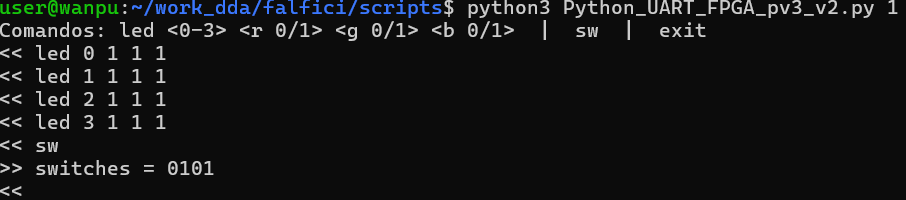
\includegraphics[width=0.5\textwidth]{imagenes/commands01.png}
        \caption{Ejmplo Nº1 de uso de los comandos definidos.}
        \label{fig:commands01}
    \end{figure}
    Donde se puede ver que se activan los 4 leds, en todos los colores posibles y se lee el valor del switch de la placa.
    \begin{figure}[H]
        \centering
        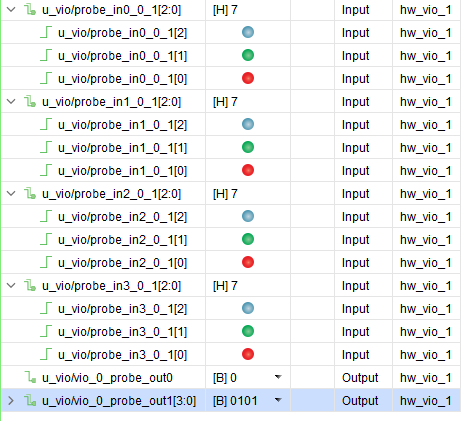
\includegraphics[width=0.4\textwidth]{imagenes/vio01.png}
        \caption{Salida obtenida en VIO.}
        \label{fig:vio01}
    \end{figure}

    \begin{figure}[H]
        \centering
        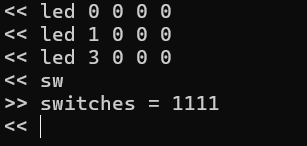
\includegraphics[width=0.4\textwidth]{imagenes/commands02.png}
        \caption{Ejmplo Nº2 de uso de los comandos definidos.}
        \label{fig:commands02}
    \end{figure}
    Donde se puede ver que se apagan los leds 0, 1 y 3, dejando el 2 encendido en su estado anterior, es decir, RGB activados.
    Nuevamente se lee el valor de los switches, pero en este caso se realizó un cambio mediante el VIO.
    \begin{figure}[H]
        \centering
        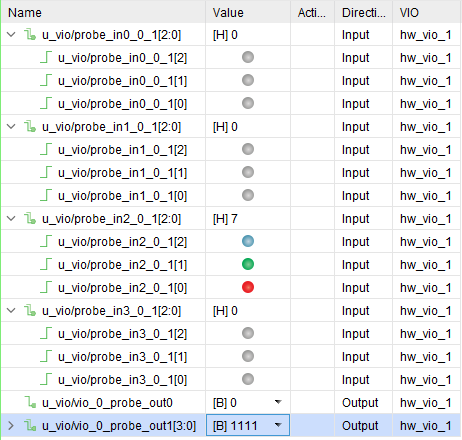
\includegraphics[width=0.4\textwidth]{imagenes/vio02.png}
        \caption{Salida obtenida en VIO.}
        \label{fig:vio02}
    \end{figure}

    \begin{figure}[H]
        \centering
        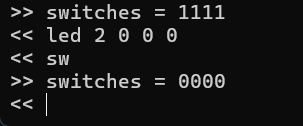
\includegraphics[width=0.4\textwidth]{imagenes/commands03.png}
        \caption{Ejmplo Nº3 de uso de los comandos definidos.}
        \label{fig:commands03}
    \end{figure}
    Finalmente, se apaga el ultimo led encendido y se deja el estado de los switches en 0.
    \begin{figure}[H]
        \centering
        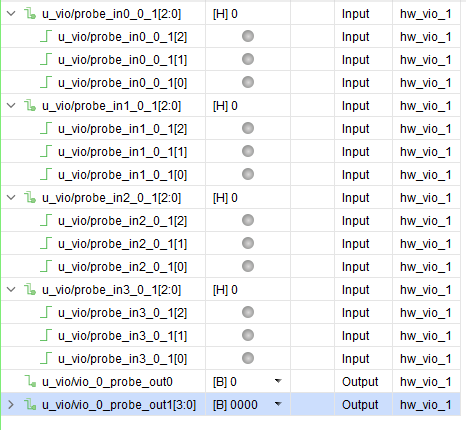
\includegraphics[width=0.4\textwidth]{imagenes/vio03.png}
        \caption{Salida obtenida en VIO.}
        \label{fig:vio03}
    \end{figure}

\newpage

\section{Conclusión}
    Como conclusión, se cierra este informe destacando la dificultad inicial de manejar el entorno de \textbf{Vitis} y la consola \textbf{XSDB}, aunque no se tuvieron mayores problemas que ese.
    El programa envía y recibe las tramas correctamente, lo que permitirá futuras implementaciones de control de la placa mediante el puerto serial de Python y el \textbf{Protocolo UART} de la 
    FPGA. Se destaca la \textbf{robustez} del sistema ante cualquier error de comunicación, ya que si se pierde la sincronización de la trama, el MicroBlaze descarta la trama y espera la siguiente,
    evitando errores en el control de los leds y switches.
\end{document}